\documentclass[9pt,aspectratio=169]{beamer} 
%设置为 Beamer 文档类型,字体为 9pt,长宽比为16:9
\usepackage{xeCJK} %导入中文包
% Beamer样式的命令和预览可参考:https://mpetroff.net/files/beamer-theme-matrix/
\setCJKmainfont{SimHei} %中文字体采用黑体
\usetheme{CambridgeUS} %选择主题,主题主要控制的是幻灯片的整体布局和配色方案。推荐最常用的五个主题:AnnArbor、CambridgeUS、Dresden、Warsaw、Berkeley。
\useoutertheme{default} %选择外部主题,外部主题主要控制的是幻灯片顶部尾部的信息栏、边栏、图标、帧标题等一帧之外的格式。预设的外部主题有:infolines、miniframes、smoothbars、sidebar、split、tree等。
\useinnertheme{default} %选择内部主题,主要控制的是标题页、列表项目、定理环境、图标环境、脚注等再一帧之内的内容格式。预设的内部主题有:circles、rectangles、rounded、inmargin等。
\usecolortheme{beaver} %选择颜色主题,颜色主题主要控制的是幻灯片的颜色搭配方案。预设的颜色主题有:albatross、beetle、crane、dolphin、fly、seagull、seahorse、whale等。
\usefonttheme[onlymath]{serif}
\usepackage[T1]{fontenc} % 让数学字体好看
\usepackage{amsmath}%常用的数学宏包
%\usepackage{amssymb}%数学宏包,可以实现一些数学符号
% \usepackage{graphicx}
% \usepackage{float}
% \RequirePackage{caption}
% \usepackage{subfigure}
% \usepackage{fancyhdr}
% \usepackage{listings}
% \usepackage{pxfonts}
% \usepackage{geometry}
\usepackage{setspace}
% \usepackage{amsfonts}%数学字体宏包
% \usepackage{comment}%批量注释的宏包
% \usepackage{boxedminipage}%为文本段添加边框的宏包
% \usepackage{shadow}%带阴影的边框
% \usepackage{fancybox}%实现边框效果的宏包
% \usepackage{esint}%实现多重积分的宏包
% \usepackage{relsize}%提供加大数学符号命令\mathlarger


\title{一个开箱即用的上海交通大学XeLatex beamer模板}
\subtitle{}
\date{\today}
\author{答辩人:XX}
\titlegraphic{
\includegraphics[width=2cm]{school_logo.png}} % 学校Logo

% 自定义文字大小和间距
\setbeamerfont{frametitle}{size=\Large,series=\bfseries}
\setbeamerfont{block title}{size=\normalsize}
\setbeamersize{text margin left=15pt,text margin right=15pt}

% 自定义定理环境
\setbeamertemplate{theorems}[numbered] %定理环境编号
\newtheorem{thm}{定理}
\newtheorem{defi}{定义}
\newtheorem{lem}{引理}
\newtheorem{assumption}{假设}

% 自定义命令
\newcommand{\any}{\forall \ }
\newcommand{\exi}{\exists \ }
\newcommand{\sothat}{\,\,\mathrm{s.t.}\,\,}

\begin{document}
\begin{frame}
	\titlepage
\end{frame}
% 首先是研究背景。我们知道,求解大规模优化问题,最经典的算法就是SGD。
\begin{frame}
\frametitle{研究背景}
考虑大规模优化问题$\min_{x\in D} f(x):=\frac{1}{m}\sum_{i=1}^{m}f_i(x).$%($D$为紧凸集,$f_i$为可微或凸函数)。
\begin{block}{随机梯度下降法(SGD):用$\nabla f$的一个无偏估计来代替$\nabla f$}
	% SGD和梯度下降法的不同之处就在于,计算梯度的时候,SGD没有直接计算$\nabla f$,而是用$\nabla f$的一个无偏估计来代替。
	对$k\in \mathbb{N}_+$,选取梯度计算式$g(x^k,a_k) \,\,\mathrm{s.t.}\,\,\mathbf{E}(g(x^k,a_k)|x^k)=\nabla f(x^k)$
,执行
	\begin{equation}
		x^{k+1}=P_D(x^k-\eta_k g(x^k,a_k))
	\end{equation}
	其中$\eta_k>0$为每次迭代时的步长,$P_D$表示到定义域的投影。
\end{block}
% 这里我们给出的是SGD的一般形式,之后我们所介绍的算法也有类似的一般形式,
% 不过为了表述方便,我们还是主要考虑定义域为$\mathbb{R}^{n}$,
% 随机梯度,从$\nabla f_1$一直到$\nabla f_m$里面均匀选取,的情况。
\vspace{0.2cm}
在后文中,我们主要考虑$D=\mathbb{R}^{n},\,g(x^k,a_k)=\nabla f_{a_{k}}\left(x^{k}\right),\,a_k \sim U (\{1,\cdots,m\})$
的情况。
\vspace{0.3cm}
% 相比于传统的梯度下降法,SGD运算效率高、内存占用小。
% 但它依然有对步长选取敏感、在病态问题中收敛缓慢等等的缺陷。
% \pause
\begin{itemize}
	\item SGD的优点:运算效率高、内存占用小;
	\item SGD的缺陷:对步长选取敏感、在病态问题中收敛缓慢、%以及
	在每个维度都采取相同步长,没有考虑不同维度上$f$的不同性质。	
\end{itemize}

\end{frame}

\begin{frame}
% 因此,我们可以考虑下面的改进算法。首先是AdaGrad-Norm.
考虑大规模优化问题$\min_{x\in \mathbb{R}^{n}} f(x):=\frac{1}{m}\sum_{i=1}^{m}f_i(x)$.
% \begin{equation*}
% 	\min_{x\in \mathbb{R}^{n}} f(x):=\frac{1}{m}\sum_{i=1}^{m}f_i(x)
% \vspace{-0.4cm}\end{equation*}
\begin{block}{AdaGrad-Norm算法:通过在分母累积历史梯度范数的平方,实现步长的自适应}
	对$k\in \mathbb{N}_+$,随机等可能地选取$a_k\in \{1,2,\cdots,m\}$,执行
	\begin{equation}\label{adagradnormdiedaigeshi}
		\begin{aligned}
		 G^{k}=G^{k-1}+\left\|\nabla f_{a_k }(x^k) \right\| _2^2,\quad
		 x^{k+1}=x^k-\frac{\eta \nabla f_{a_k}(x^k) }{\sqrt{G^k+\varepsilon}}.
		\end{aligned}
	 \end{equation}
	 其中$G^0=0,\,\eta>0$为初始步长,$\varepsilon\approx 10^{-7}$为数值稳定性小量。
\end{block}
% 这个算法通过在分母累积历史梯度范数的平方,来实现步长的自适应。
% 可以看出,在梯度比较小,函数较为平缓的时候,算法会保持较大步长,否则算法的步长就会迅速减小。
% 
% 而AdaGrad可以看成是逐分量的AdaGrad-Norm. 
\begin{block}{AdaGrad算法 (John Duchi et al. 2011):逐分量的AdaGrad-Norm}
		对$k\in \mathbb{N}_+$,随机等可能地选取$a_k\in \{1,2,\cdots,m\}$,执行
		\begin{equation}\label{adagraddiedaigeshi}
			\begin{aligned}
			 G^{k}=G^{k-1}+\nabla f_{a_k }(x^k)\odot \nabla f_{a_k }(x^k) ,\quad
			 x^{k+1}=x^k-\frac{\eta  }{\sqrt{G^k+\varepsilon}}\odot \nabla f_{a_k}(x^k).
			\end{aligned}
		 \end{equation}
		 其中$G^0=\mathbf{0},\,\eta>0,\,\varepsilon\approx 10^{-7}$,除法、根号、加法均视为逐分量运算。
\end{block}
\vspace{0.3cm}
% 这里的odot记号代表哈达玛积,也就是对向量的每个分量单独做乘法,得到一个新的向量。这里的$G^k$加e就是每个分量都加上e,
% 根号和除法也是对每个分量单独计算。
AdaGrad在病态问题和稀疏数据上表现较好,逐分量自适应步长是关键。
% 之后我们将会看到,AdaGrad在病态问题和稀疏的数据集上表现比较好,但是同样是自适应步长的AdaGrad-Norm表现
% 就没那么好,原因是,这里的逐分量自适应步长的操作,起了关键的效果。
\end{frame}
% 接下来我们介绍AdaGrad的理论性质。AdaGrad主要应用于 随机优化 和 在线学习 。
% 关于它的理论性质的研究,也主要基于这两种情境。 
\begin{frame}
	\frametitle{AdaGrad的理论性质(随机优化情境)}
% 在随机优化情境下,我们有下面的收敛结果。
\vspace{-0.3cm}
\begin{thm}[光滑非凸情境中的收敛速度]
	用AdaGrad算法\,(\ref{adagraddiedaigeshi})\,\,求解大规模优化问题$\min_{x\in \mathbb{R}^{n}} f(x):=\frac{1}{m}\sum_{i=1}^{m}f_i(x)$,如果
	\\ \vspace{0.2cm} 假设1:目标函数下有界:$\any x\in \mathbb{R}^{n},\,f(x)\geq f_{*}$;
\\ \vspace{0.1cm} 假设2:随机梯度一致有界:
    $\exi M,\,\sothat \any 1\leq i\leq m,\,\any x\in \mathbb{R}^{n},\,\left\| \nabla f_{i}(x) \right\|_\infty \leq M$;
\\ \vspace{0.1cm} 假设3:目标函数L-光滑:
  $\any x,y\in \mathbb{R}^{n},\,\left\| \nabla f(x)-\nabla f(y) \right\|_2 \leq L \left\| x-y \right\|_2 $,
 \\ \vspace{0.15cm} 则在$T-1$次迭代后,从迭代点列$\{x^k\}_{k=1}^T$中随机选取一个点作为输出,该点处目标函数的梯度值的期望至多与$\ln T/T$同阶:
	\begin{equation}\label{zhuyaojieguo}
		\mathbf{E}_{t}\left( \left\|\nabla f(x^{t}) \right\|_2^2 \right) :=\mathbf{E}\left( \frac{1}{T}\sum_{k=1}^{T}\left\|\nabla f(x^{k}) \right\|_2 ^2\right) =O \left( \frac{\ln T }{T} \right).
	\end{equation}
\end{thm}
% 定理的证明主要是利用L-光滑函数的二次上界
\begin{block}{Proof (sketch).}
	设$x^{k+1}=x^k-\eta u_k,\,\,u_k=\nabla f_{a_k}(x^k)\odot (1 /\sqrt{G^k+\varepsilon})$,
	利用L-光滑函数的二次上界可见
	\begin{equation}\label{untitle6}
        f(x^{k+1})\leq f(x^k)-\eta u^k\cdot \nabla f(x^k)+ \frac{L}{2}\left\| \eta u^k \right\|_2 ^2,
    \end{equation}
\end{block}
\end{frame}

% 以及条件期望的性质。
% 并且,这个证明是基于一般的随机优化情境的,也就是说,我们只用到了
% 随机梯度是真实梯度的无偏估计这个条件,并不一定要从fi里面随机均匀选取一个来计算梯度。
\begin{frame}
	\begin{proof}[]
		用$\mathbf{E}_{i}\left(\,\cdot\, \right)$表示条件期望$\mathbf{E}\left(\,\cdot \,|\,a_1,\cdots,a_i\right),\,\mathbf{E}_0\left(\,\cdot\,\right):=\mathbf{E}\left(\,\cdot\,\right)$,上式两端求条件期望可见
		\vspace{-0.05cm}\begin{align}\label{untitle7}
		\mathbf{E}_{k-1}\left( f(x^{k+1})\right)& \leq f(x^k)-\eta\mathbf{E}_{k-1}\left( u^k\cdot \nabla f(x^k)\right)+ \frac{L\eta^2}{2}\mathbf{E}_{k-1}\left(\left\|  u^k \right\|_2 ^2\right).
		\vspace{-0.1cm}\end{align}
 $\mathbf{E}_{k-1}\left( u^k\cdot \nabla f(x^k)\right)$表示更新方向与负梯度方向的平均偏差,
具有下界	\vspace{-0.15cm}\begin{equation}
	\mathbf{E}_{k-1}\left(\nabla f(x^k)\cdot u^k\right)\geq \frac{\left( \nabla  f(x^k) \right) ^2}{2\sqrt{kM^2+\varepsilon}}-2M \mathbf{E}_{k-1}\left(\left\| u^k  \right\|_2 ^2\right),
\vspace{-0.05cm}\end{equation}
将其代入\,(\ref{untitle7})\,,对$k=1,2,\cdots,T$求和后,两端再求期望。
由条件期望的性质,对$k\in \mathbb{N}_+$有
$\mathbf{E}\left(\mathbf{E}_{k-1}\left( \,\cdot\,\right)\right)=\mathbf{E}\left(\,\cdot\,\right)$,可见
\vspace{-0.2cm}\begin{equation}\label{qiuheshi2}
	\mathbf{E}\left(f(x^{T+1})\right)\leq \mathbf{E}\left(f(x^1)\right)+
	\sum_{k=1}^{T}\left( -\frac{\eta \mathbf{E}\left(\left\| \nabla f(x^k) \right\|_2 ^2\right)}{2M_1}+ C\mathbf{E}\left(\left\|  u^k \right\|_2 ^2\right)   \right).
	\vspace{-0.2cm}\end{equation}
	其中$C= 2M\eta+ \frac{L\eta^2}{2},\,M_1=\sqrt{TM^2+\varepsilon}$.\ 最后再说明
	\vspace{-0.05cm} \begin{equation}\label{untitle9}
        \sum_{k=1}^{T}\mathbf{E}\left(\left\|u^k \right\|_2 ^2\right)
\leq \sum_{j=1}^{n}\mathbf{E}\left(\ln \left( 1+\frac{\sum_{s=1}^{T}\left( g_j^s \right) ^2}{\varepsilon} \right) \right)
\leq   n \ln \left( 1+\frac{TM^2}{\varepsilon} \right),
\vspace{-0.05cm}\end{equation}
代入整理可得欲证结论。
\end{proof}

\end{frame}
\begin{frame}
	\frametitle{AdaGrad的理论性质(在线学习情境)}
% 对于AdaGrad在在线学习情境下的理论性质,我们有下面的收敛结果。
\begin{thm}[凸优化情境下的收敛率]
	用AdaGrad算法\,(\ref{adagraddiedaigeshi})\,\,求解
	大规模优化问题$\min_{x\in D} f(x):=\frac{1}{m}\sum_{i=1}^{m}f_i(x)$,如果
	\\ \vspace{0.2cm} 假设1:$D$为紧凸集,$f_1,\cdots,f_m$为凸函数,且$f$存在最小值点$x^{*}\in D$;
	% 同时
	\\ \vspace{0.1cm} 假设2:随机(次)梯度一致有界:$\any x\in D,\,i\in \{1,\cdots,m\}$,有$\left\| \nabla f_i(x) \right\|_\infty \leq M $,
	\\ \vspace{0.1cm} 
	\setstretch{1.2}
	则在$T-1$次迭代后,采用迭代点列的平均值作为输出,将得到期望意义下$O(1/\sqrt{T})$的收敛率。
	具体而言,记$\bar{x}_T=\frac{1}{T}\sum_{i=1}^{T}x^t$,$d=\sup_{x,y\in D,\,1\leq j\leq n} \left| x_j-y_j \right| $,则
	\vspace{-0.2cm}\begin{equation}
		\mathbf{E}\left(f(\bar{x}_T)-f(x^{*})\right)\leq \frac{n}{T} \sqrt{TM^2+\varepsilon} \left( \frac{d^2}{2\eta}+\eta \right).
\end{equation}
\end{thm}
% 定理的证明主要利用了AdaGrad的遗憾界,以及遗憾界限与算法收敛率的关系。
\begin{proof}[Proof (sketch)]
	只需证明AdaGrad具有与随机梯度选取无关的遗憾界
    \vspace{-0.2cm}\begin{equation}
       % R(T)\leq \sum_{j=1}^{n}\left( \sqrt{T} \left( \frac{d_j^2}{2\eta}+\eta  \right) +\frac{2d_j^2\varepsilon}{\eta} \right) 
        R(T)\leq B(T)=\sum_{j=1}^{n} \sqrt{TM^2+\varepsilon} \left( \frac{d_j^2}{2\eta}+\eta  \right),
   \vspace{-0.2cm} \end{equation}
    其中$d_j=\sup_{x,y\in D}\left| x_j-y_j \right|$.\ 再利用遗憾的性质证明$\mathbf{E}(f(\bar{x}_T)-f(x^{*}))\leq \frac{B(T)}{T}$即可。
\end{proof}
\end{frame}
% 遗憾是在线学习里面一个重要的概念,
\begin{frame}
考虑大规模优化问题$\min_{x\in D} f(x):=\frac{1}{m}\sum_{i=1}^{m}f_i(x),\,$其中
$D$为紧凸集,诸$f_i$为凸函数。
\begin{defi}[遗憾]
设某随机梯度方法第$k$次迭代起始点为$x^k$,所选取的随机(次)梯度为$\nabla f_{a_i}(x^k)$,称
\begin{equation}\label{yihandingyi}
    R(T)=\sum_{i=1}^{T} f_{a_i}(x^i) -\min_{x\in D}\sum_{i=1}^{T} f_{a_i}(x) 
\end{equation}
为该方法迭代$T$轮所产生的\textbf{遗憾}(\textrm{regret}\,).\ 遗憾代表在线算法的总损失与离线算法的理论最小损失之间的差值。
\end{defi}
\vspace{0.2cm}

当随机梯度一致有界时,我们有
\vspace{0.2cm}
\begin{itemize}
	% 如果合适地选取步长,
	\item 取步长$\eta_k=\eta/\sqrt{k}\,\,(\eta>0)$,此时SGD具有遗憾界$R(T)\leq B(T)=O(\sqrt{T})$;
	\item 对任意初始步长,AdaGrad和AdaGrad-Norm具有遗憾界$R(T)\leq B(T)=O(\sqrt{T})$;
    \item AdaGrad和AdaGrad-Norm的最优遗憾界为后见之明意义下最优遗憾界的$\sqrt{2}$倍。
\end{itemize}

\end{frame}
\begin{frame}
	\frametitle{Ada-系列算法}
% AdaGrad算法最主要的缺点是:
受历史梯度累积影响,AdaGrad步长递减趋于0,导致迭代后期收敛缓慢,对新数据的学习能力较弱。
% 要克服这个缺陷的话,我们可以考虑
\begin{block}{RMSProp:将记录梯度的二阶矩的$G^k$改为指数滑动平均的形式}
	% 这样算法就能遗忘较远的梯度信息。
	\begin{equation}\label{RMSPropdiedaigeshi}
        \begin{aligned}
            G ^k&=\rho G^{k-1}+(1-\rho)(\nabla f_{a_k}(x^k)\odot \nabla f_{a_k}(x^k)) &\\ 
          x^{k+1}&=x^k- \frac{\eta }{\sqrt{G^k+\varepsilon}} \odot \nabla f_{a_k}(x^k), & k=1,2,\cdots,
		\end{aligned}
      \end{equation}
      其中$G^0=\mathbf{0}$,$\rho\in(0,1)$为衰减参数,一般取$0.9$.\ 
\end{block}
\begin{block}{Adam:在RMSprop的基础上引入动量,并进行偏差修正}
	% 同时,我们可以考虑引入动量来加速收敛。
	% 具体来说,就是在确定当前更新方向的时候,对上次迭代的前进方向和当前选取的随机梯度方向做一个加权平均。
	\begin{equation}
		\begin{aligned}
			S^{k}&=\rho_1 S^{k-1}+(1-\rho_1) \nabla f_{a_k}(x^k),  \\
			G^k&=\rho_2 G^{k-1}+(1-\rho_2)\nabla f_{a_k}(x^k)\odot \nabla f_{a_k}(x^k), \\ 
			\hat{S}^k&=\frac{S^k }{1-\rho_1^k},\,\,\hat{G}^k=\frac{G^k }{1-\rho_2^k}, \\ 
			x^{k+1}&=x^k- \frac{\eta }{\sqrt{\hat{G}^k+\varepsilon}} \odot \hat{S}^k, & k=1,2,\cdots.
		\end{aligned}
	\end{equation}	
其中$S^0=G^0=\mathbf{0}$,衰减参数$\rho_1,\,\rho_2\in(0,1)$,一般取$\rho_1=0.9,\,\rho_2=0.999$.
% 在论文的第三章,我们主要介绍了。。。这些改进算法。AdaGrad和这些改进算法一般统称为Ada-系列算法。
\end{block}
\end{frame}

\begin{frame}
	\begin{columns}
		\column{0.5\textwidth}
		\LARGE 数值实验
\vspace{0.3cm}
		\normalsize
		\begin{itemize}
			\item {
				考虑对应了三类优化问题(光滑强凸、非光滑凸、光滑非凸)
				的三种模型(Logistic回归(LR)、支持向量机(SVM)、多层感知机(MLP));
			}
			\item {数据集:Ads(稀疏)、Spambase(非稀疏);}
			\item {算法:SGD, AdaGrad, AdaGrad-Norm, RMSProp, AdaDelta 和 Adam;}
			\item {主要结论:\\ 
			Ada-系列算法的整体表现较好,在稀疏数据集Ads上,差距更加明显。}
			\vspace{0.3cm}
		\end{itemize}\
		右图是在稀疏数据集Ads上,用各种算法训练LR模型,迭代100轮后的结果。蓝色、红色、绿色线分别表示验证准确度、精确度、召回率。
		% \bigskip
		% \bigskip
		% \bigskip
		% \bigskip
		% \bigskip
		% \bigskip
		\column{0.5\textwidth}
	\begin{figure}
			\centering
			% Requires \usepackage{graphicx}
			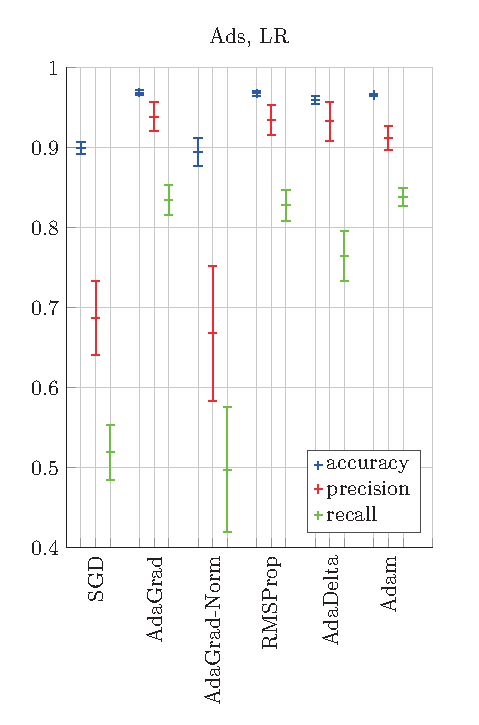
\includegraphics[width=5.1cm]{image/1new.eps}
	\end{figure}
\end{columns}
\end{frame}

\begin{frame}
	\frametitle{总结与展望}
SGD与Ada-系列算法各自的优缺点:
\begin{itemize}
	%对Ada-系列算法各自的优点、缺点进行总结,并与SGD作比较;
	\item SGD超参数少、可解释性强、泛化能力好,但在病态问题中收敛慢、对步长敏感、难以逃脱鞍点;
	\item AdaGrad适合稀疏数据、在病态问题下收敛快、无需手动调整步长,但其步长单减趋于0,迭代后期收敛缓慢,对新数据的
	学习能力较弱;
	\item RMSProp, AdaDelta, Adam 等改进算法避免了步长过早衰减、对新数据学习能力较强、对不同模
	型和超参数的鲁棒性强,但迭代格式较复杂,缺乏收敛性的理论保证,并且在神经网络等模型中泛化能力可能较弱。
\end{itemize}
\vspace{0.3cm}
Ada-系列算法适合稀疏数据的关键因素:逐分量自适应步长。
如果某个特征很少出现,那么在该特征对应的分量上,梯度的累积将很少,因此 Ada-系列算法能在
特征出现时作出及时的反应(在该方向给予一个较大步长)。


\vspace{0.3cm}
论文关于AdaGrad收敛性刻画的不足之处:
\begin{itemize}
	\item 在凸优化问题中,$O(1/\sqrt{T})$的收敛率与定义域直径有关;
	\item 在光滑非凸优化问题中,刻画收敛性的指标不如收敛率直接,并且$O(\ln T/\sqrt{T})$的收敛速度与问题维数$n$、数值稳定性小量$\varepsilon$有关。
\end{itemize}
	

\end{frame}
\end{document}